\documentclass[a4paper, 11pt]{article}

\usepackage[utf8]{inputenc}
\usepackage[T1]{fontenc}

\usepackage[left=2cm, right=2cm, top=2cm, bottom=2cm]{geometry}

\usepackage{graphicx}

\usepackage{listings}
\usepackage{xcolor}

\usepackage{amsmath}
\usepackage{amssymb}

\include{graphix}

\lstset{frame=tb,
  language=Python,
  aboveskip=3mm,
  belowskip=3mm,
  showstringspaces=false,
  columns=flexible,
  basicstyle={\small\ttfamily},
  numbers=none,
  numberstyle=\tiny\color{gray},
  keywordstyle=\color{blue},
  commentstyle=\color{brown},
  stringstyle=\color{black},
  breaklines=true,
  breakatwhitespace=true,
  tabsize=4
}


\title{ExoGravity Tutorial}
\author{Mathias Nowak}
\date{\today}

\begin{document}
\maketitle

\section{A quick overview of the data}

Let's start this tutorial with a quick overview of what the GRAVITY data look like. The document only deal with dual-field data (as opposed to single-field), at the ``astrored'' reduction level (so, not the fully pipeline-reduced ``scivis'' data). There are a couple of important differences between ``astrored'' data and ``scivis'': in the ``astrored'', the DITs are kept separate, whereas to create the ``scivis'', the pipeline average them; and in ``astrored'' files, the phase of the visibility is not corrected for fringe-tracker referencing, dispersion correction, non-common path error correction, etc.). The exoGravity pipeline is based on those dual-field astrored data products.

Two example data file are provided with this tutorial, which correspond to the same exposure made on 51~Eri, during the night of Nov, 11, 2019. The difference between those two files is that one of them contains a few extra corrections data.
\begin{itemize}
\item{Pipeline reduced ``astrored'': \verb|GRAVI.2019-11-11T06:29:03.495_astroreduced.fits|}
\item{With additional info from Sylvestre: \verb|GRAVI.2019-11-11T06:29:03.495_astroreduced_s.fits|}
\end{itemize}

To look at what is inside these data files, you can open one of them files with ``fv''\footnote{https://heasarc.gsfc.nasa.gov/ftools/fv/} (see Figure~\ref{fig:fv})

\begin{figure}
  \begin{center}
    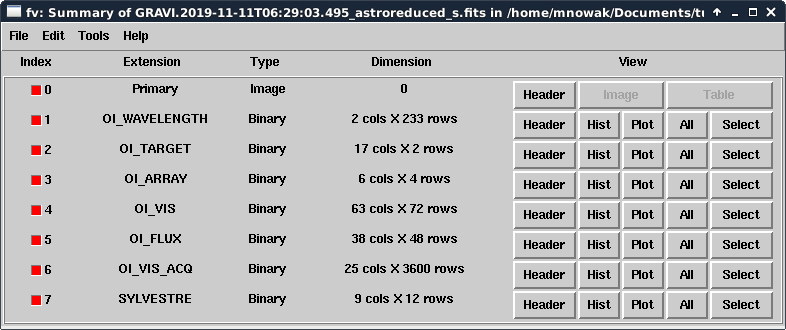
\includegraphics[width=\linewidth]{figures/fv.png}
    \caption{A GRAVITY data file opened with ``fv'', where the different OIs contained in the FITS file are displayed.}
    \label{fig:fv}
  \end{center}
\end{figure}

Each file is divided in different ``OIs'', which contain different fields. Here are the data which are the most useful for exoGravity:
\begin{itemize}
\item{Primary header: The main header contains several useful inforoamtion. Some of the not-so-obvious are: \verb|SOBJ X| and \verb|SOBJ Y|, which give the position of the science fiber with respect to the FT fiber (RA/DEC, in mas); \verb|SOBJ SWAP| tells whether or not the exposure is done at the swapped position; \verb|DET2 SEQ1 DIT| and \verb|NDIT OBJECT| give the integration time (for one DIT, in s), and the number of DITs in the exposure file}
\item{\verb|OI_WAVELENGTH|: \verb|EFF_WAV| contains the wavelength grid, in meters}
\item{\verb|OI_TARGET|: Not used}
\item{\verb|OI_ARRAY|: Not used}
\item{\verb|OI_VIS|: contains the visibiliy (or baseline-based) data. In particular, \verb|VISDATA| contain the complex raw visibilities as extracted by the pipeline, and \verb|VISERR| contain the error on the real and imaginary parts of the \verb|VISDATA|. \verb|UCOORD| and \verb|VCOORD| contain the UV coordinates of the baselines, in meters. \verb|PHASE_REF| contains the phase reference point of the Fringe-Tracker, and \verb|OPD_DISP| contain the OPD dispersion correction}
\item{\verb|OI_FLUX|: contains the flux data, and some important telescope-based quantities related to the metrology correction. \verb|FLUX| and \verb|FLUXERR| give the flux and the associated error bars. The two quantities \verb|OPD_MET_TELFC_MCORR| and \verb|OPD_MET_FC_CORR| are used for the metrology correction (non-common path errors)}
\item{\verb|OI_VIS_ACQ|: Not used}
\item{\verb|SYLVESTRE|: only present in the \verb|_s.fits| file, this extension contains data used for alternative OPD dispersion and metrology corrections}
\end{itemize}



\section{The cleanGravity package}

\subsection{Load a file}

To simplify the manipulation of the data, a dedicated package is provided with the exoGravity pipeline: \verb|cleanGravity|. The aim of that package is to provide an Python object-oriented interface to the GRAVITY data.

Different classes are defined, to fit the specificity of the different GRAVITY file products:
\begin{itemize}
\item{\verb|GravityDualscivisAstrored|}
\item{\verb|GravitySinglefieldsAstrored|}
\item{\verb|GravityDualfieldScivis|}
\item{\verb|GravitySinglefieldScivis|}
\end{itemize}

In the exoGravity pipeline, only \verb|GravityDualfieldAstrored| objects are used. The syntax to load a file into on of these objects is always similar. In the most basic form, you only need to specify the name of the FITS file to load, as well as the extension (when you have different polarizations, you have different extensions): 
\lstinputlisting[linerange={1-3}]{../python/data_manipulation.py}

\noindent{}When the \verb|GravityOi| object is created, several attributes are created:
\begin{itemize}
\item{\verb|oi.header| is an astropy object, which contain the main header}
\item{\verb|oi.visOi| contains the data from the \verb|OI_VIS|. It is a \verb|visOi| object, as defined in the \verb|cleanGravity| package}
\item{\verb|oi.fluxOi| contains the data from the \verb|FLUX_VIS|, in a \verb|fluxOi| object}
\item{Several useful attributes are also loaded from the header, like \verb|oi.sObjX| and \verb|oi.sObjY| (position of the fiber), \verb|oi.mjd| (time of observation), etc. Please refer to the documentation of the package}
\end{itemize}

Once the \verb|GravityOi| object is created, the different data sets are automatically loaded and reshaped in numpy arrays, complex or reals (depending on the data). The shape of these arrays is always:
\begin{equation*}
\text{Shape of the numpy data arrays in cleanGravity:} \qquad \left[n_\mathrm{DIT}, n_\mathrm{channels}, n_\mathrm{wav}\right]
\end{equation*}
\noindent{}Where $n_\mathrm{DIT}$ is the number of DITs in the exposure file, $n_\mathrm{channels}$ the number of channels in the OI (4 channels corresponding to 4 telescopes in the \verb|FLUX_OI|, 6 channels for 6 baselines in \verb|VIS_OI|), and $n_\mathrm{wav}$ corresponds to the number of wavelength points.

\noindent{}For example:
\lstinputlisting[linerange={5-6}]{../python/data_manipulation.py}

\noindent{}As another example, you can plot the flux on each telescope as a function of wavelength using something like:
\lstinputlisting[linerange={8-17}]{../python/data_manipulation.py}

\subsection{Plotting with gravityPlot}

The visibility data contained in \verb|oi.visOi.visData| are complex numbers. To plot them, you need to separate real/imaginary, modulus/phase, or use 3D graphs. To make things easier for a quick view at the data, the \verb|cleanGravity| also provides some plotting functions. These are not automatically loaded at the import of the package, to allow for changing the configuation of \verb|matplotlib| if needed, before importing the plot functions. You can import these functions, and plot the visibilities in real/imaginary parts using:
\lstinputlisting[linerange={19-22}]{../python/data_manipulation.py}

The \verb|modPhasePlot| function does the same thing, but in modulus/phase instead of real/imaginary parts. You can also plot a real quantity over several channels at once using the \verb|baselinePlot| function. For example, instead of looping over the telescopes to plot the flux, you can use the one-liner:
\lstinputlisting[linerange={24-25}]{../python/data_manipulation.py}


\subsection{Standard phase corrections}

The \verb|cleanGravity| package also provides methods to apply the phase corrections to the ``astrored'' data. The FT referencing is automatically applied when the data are loaded, and the resulting ``FT referenced'' visibilities are available in \verb|oi.visOi.visRef|. To apply the OPD dispersion correction, just call \verb|oi.corrDisp()|, or \verb|oi.corrDispSylvestre()|, if you want to use the Sylvestre special correction (only with a \verb|_s.fits| file). Similarly, to apply the metrology (non common path) correction, call \verb|oi.corrMet()|, or \verb|oi.corrMetSylvestre()|.

The phase corrections are always performed on the \verb|oi.visOi.visRef| arrays. The \verb|oi.visOi.visData| stays at the initial values, which give the raw visibilities.

These corrections can be automatically applied when loading the data, by setting the \verb|corrDisp| or \verb|corrMet| kwargs:
\lstinputlisting[linerange={27-28}]{../python/data_manipulation.py}



\section{An example: extracting the astrometry of a binary from a swap observation}
\label{sec:swap_example}

\subsection{Observations}
For this example, we are going to use some data obtained during an observation of HD~25535, on November, 11, 2019. The data are located in the folder \verb|HD25535/|.

The observation was carried out in \emph{dual-field} (one fiber used for the Fringe Tracker, and one for the ``science'' target), \emph{off-axis} (the roof mirror is used, and neither the FT fiber, not the science fiver, is centered in the field), using the ``swap'' template. During a swap observation, exposures are acquired sequentially with two configurations (see Figure~\ref{fig:swap}): 1- the FT fiber is centered on the target star, and the science fiber is the requested offset position; 2- the science fiber is one the target star, and the FT fiber at the given offset position compared to the science fiber (the two fibers are ``swapped'').

Note that this observation pattern can only be used for binary systems in which the two components are bright enough to feed the FT.

In the present case, a total of 8 exposures were aquired: 2 in the standard configure (FT on target), 2 in the swapped configuration (FT at offset position), then again 2 in standard configuration, and 2 in swapped configuration.

\begin{figure}
  \begin{center}
    %    \includegraphics[width=0.8\linewidth]{figures/swap.png}
    \caption{Illustration of the swap sequence}
  \end{center}
\end{figure}

The objective of the data reduction is to extract the astrometry of the binary. This is done by fitting the visibility of the science object. But to get a proper astrometry, several problems need to be taken care of:
\begin{enumerate}
\item{We are working with astrored files, so we need to take care of the FT zero point, dispersion, and metrology corrections}
\item{We are in dual-field, so we need to calculate the phase reference and to subtract it the observed visibilities}
\item{We are in swap mode, so remind that half the data are measuring $(\Delta\mathrm{RA},\Delta{}\mathrm{DEC})$, and half are measuring $(-\Delta\mathrm{RA},-\Delta{}\mathrm{DEC})$}
\end{enumerate}

\subsection{Imports}

For this section, we are going to use the \verb|cleanGravity| package, as well as the plotting functions contained in \verb|gravityPlots| (not automatically loaded), and a few standard packages.
If you want to run the examples, I suggest you import the following, and also define the \verb|DATADIR| variable to point to the HD~25535 directory.
\lstinputlisting[linerange={1-6}]{../python/swap_example.py}


\subsection{Load the data and apply the corrections}

\subsubsection{FT corrected visibilities}

Using \verb|cleanGravity|, the data can be loaded as \verb|GravityDualfieldAstrored| objects. You need to specify the path to the FITS file, and the FITS extension:
\lstinputlisting[linerange={8-9}]{../python/swap_example.py}

The attribute \verb|oi.visOi| is a \verb|VisOi| object, which contains the visibility data. The raw data can be accessed in \verb|oi.visOi.visData|. The package always takes care of correcting for the FT zero point, and the visibilities referenced to the FT are in \verb|oi.visOi.visRef|. You can easily visualize the difference between the two using the gravityPlot functions:
\lstinputlisting[linerange={11-14}]{../python/swap_example.py}

You can easily see how the FT tracking reference is shifting at each DIT by plotting the DITs individually:
\lstinputlisting[linerange={16-20}]{../python/swap_example.py}

\noindent{}Replace \verb|visData| with \verb|visRef|, and you should see that the FT corrected visibilities are now better aligned:
\lstinputlisting[linerange={22-26}]{../python/swap_example.py}


\subsubsection{OPD dispersion correction}

When working with fully reduced data (``scivis'' files), this step is taken care of by the GRAVITY pipeline. But when working with the ``astrored'' data, this correction is not applied by the pipeline. However, the OPD that needs to be added to the visibilities is calculated by the pipeline, and is available in \verb|oi.visOi.opdDisp|. So the correction is a simple one-liner:
\lstinputlisting[linerange={28-29}]{../python/swap_example.py}

\noindent{}For convenienence, this correction can also be applied directly when loading the data with \verb|cleanGravity|, simply by setting a \verb|corrDisp| keyword to \verb|"drs"| instead of the default \verb|"none"|:
\lstinputlisting[linerange={31-32}]{../python/swap_example.py}

Note that there exists an alternative calculation of the OPD dispersion correction, made by Sylvestre. This correction is applied in the same way, except that the \verb|opdDisp| values in this case are located in another OI of the FITS file (called SYLVESTRE). For the moment, this OI is not available by default in the pipeline reduced data. If you happen to have a file in which this OI is available\footnote{Usually, it means that you got it from Sylvestre himself}, you can request this alternative correction by setting \verb|corrDisp = "sylvestre"|:
\lstinputlisting[linerange={34-35}]{../python/swap_example.py}


\subsubsection{Metrology correction}

The metrology correction is also done by the pipeline on the ``scivis'' file, but not on the ``astrored'' files. Since we are working with the latter, we need to apply it manually. Again, this can be done by setting a keyword \verb|corrMet = "drs"| when loading the data:
\lstinputlisting[linerange={37-38}]{../python/swap_example.py}

But the sake of explanations, we are going to do it manually. The metrology correction comes from telescope-based measurements. This means that the required quantities must be retrieved from the flux OI, not from the visibility OI. They are available in the \verb|oi.fluxOi| object, as \verb|oi.visOi.telFcCorr| and \verb|oi.visOi.fcCorr|. The sum of the two give an OPD correction for each telescope. To convert it to a correction for each baseline, it is necessary to calculate the difference between the proper telescopes (two telescope per baseline).

In the \verb|visOi| object, the visibilities are ordered in decreasing order: $T_4$-$T_3$, $T_4$-$T_2$, $T_4$-$T_1$, $T_3$-$T_2$, $T_3$-$T_1$, $T_2$-$T_1$. The same if true for the telescopes in the \verb|fluxOi|: $T_4$, $T_3$, $T_2$, $T_1$. Thus, the conversion from telescope-based errors to baseline-based errors can be done using the following matrix:
\lstinputlisting[linerange={40-46}]{../python/swap_example.py}

With the matrix, the correction proceeds easily. You just have to remind that the values give an OPD correction, which needs to be divided by $\lambda$ to get a phase correction:
\lstinputlisting[linerange={48-50}]{../python/swap_example.py}

Again, there exists an alternate correction, which uses the SYLVESTRE OI, and which can be requested by setting \verb|corrMet = "sylvestre"| instead of \verb|"drs"|.

\subsection{Optional: calculate the mean of the DITs}

This step is optional. It is usually better to keep the DITs separated, but depending on how many files you have to reduced, and what the spectral resolution is, the computation can then be lengthy. Thus, when developing, it can be useful to average the DITs to speed up things.

Due to the rotation of the sky, averaging the visibilities is not as trivial as it sounds. The OPD on each baseline is changing with time, and thus the phase of the visibility is drifting. As a consequence, to average the visibilities properly, you first need to ``shift'' them to $\mathrm{OPD} = 0$. Ideally, this should be done using the proper astrometry of the target. Since it is unknown, the best way is to proceed using the position of the fiber as a substitue. To do that, you can use the \verb|recenterPhase| method of the \verb|visOi| object, to ``recenter'' the visbilities on the fiber position (available in RA/DEC in \verb|oi.sObjX| and \verb|oi.sObjY|). Then you can average the visibilities, the baselines UV coordinates, and shift the visibilities back to their original position:
\lstinputlisting[linerange={52-63}]{../python/swap_example.py}

Note that in the above code, the use of the \verb|np.tile| functions guarantees that the visibility data keep the same format (3 dimensional arrays, first dimension for the DIT number, second for the channel, and third for the walength).

\subsection{Separate and average the swap positions and calculate the phase reference}

At this point, you have the visibilities referenced to the FT, properly corrected for the dispersion, and for the metrology (i.e. for non common-path errors). Potentially, you have also averaged those visibilities. But these visibilities are still corrupted by the unknown metrology zero point (i.e. the phase picked up at the injection of the metrology laser in the system). Fortunately, this phase error is extremely stable. This means that, as long as you did not switched the observing mode (on-axis/off-axis) between the different exposures, this phase offset will be the same in all the data.

\noindent{}Consequently, for a swap observation, the phase at the two positions are respectively given by:
\begin{align*}
\text{Before the swap:} \qquad & \phi(u, v) = \frac{2\pi}{\lambda}\left(\Delta\mathrm{RA}\times{}u+\Delta\mathrm{DEC}\times{}v\right) + \phi_\mathrm{ref} \\
\text{After the swap:}  \qquad & \phi_\mathrm{swap}(u, v) = \frac{2\pi}{\lambda}\left(-\Delta\mathrm{RA}\times{}u-\Delta\mathrm{DEC}\times{}v\right) + \phi_\mathrm{ref}  
\end{align*}

\noindent{}Calculating the phase reference is thus just a matter of summing the phase of the two positions:
\begin{equation*}
  \phi_\mathrm{ref} = \frac{\phi + \phi_\mathrm{swap}}{2}
\end{equation*}

\noindent{}So the sequence to retrieve the phase reference is the following:
\begin{enumerate}
\item{Load all the files, and correct the visibilities referenced to the FT for dispersion and metrology}
\item{Separate the OIs in two groups: standard and swapped. This can be done using the \verb|oi.swap| boolean}
\item{Average the visibilities over each of the two groups, and extract the phase\footnote{The instrument measures the real and imaginary parts of the visibilities, not the phase. So you should always average the visibilities first and calculate the phase after! Never do the opposite (calculate the phase and then average).}}
\item{Calculate the phase reference}
\item{Subtract this phase reference to the visibilities of each file} 
\end{enumerate}
  
\noindent{}In Python, this goes as follows. First, all files are loaded and separated in two groups with:
\lstinputlisting[linerange={66-75}]{../python/swap_example.py}

\noindent{}Then, the average on each group can be calculated, again by first shifting the visibilities to 0 OPD:
\lstinputlisting[linerange={77-87}]{../python/swap_example.py}

\noindent{}The phase reference is extarcted and removed from all the OIs:
\lstinputlisting[linerange={89-92}]{../python/swap_example.py}



\subsection{Fit for the astrometry}

From there on, the visibility you have in \verb|oi.visOi.visRef| should correspond to the astrophysical visibilities. The last thing to do is to fit for the astrometry of the binary.

A simple model for the visibilities, with two free parameters $\Delta\mathrm{RA}$ and $\Delta\mathrm{DEC}$ can be built from the following equation, which gives the visibility as a function of the baseline coordinates:
\begin{equation*}
  V_{(\Delta{}\mathrm{RA}, \Delta{}\mathrm{DEC})}(U, V) = |V|\exp\left\{{i\,2\pi}\left(\Delta\mathrm{RA}\times{}U+\Delta\mathrm{DEC}\times{}V\right)\right\}
\end{equation*}
\noindent{}In which $|V|$ is a visibility modulus.

A basic fit of this model could be a linear fit, in which a scaling factor is adjusted for each baseline and each DIT, to take into account the variations in the transmission. It should be noted, though, that you should never let the scaling factor be negative. A negative scaling factor can ``revert'' the fringes, making a completely out-of-phase model (i.e. with a phase offset of $\pi$ compared to the data) look ``good''. One simple strategy is to operate a linear fit, and if the resulting scaling coefficient is negative, set it to 0. Alternatively, if the model include other elements, for example an underlying polynomial to model a contamination on the detector, you could set the wavelet (the visibility model) to 0, and redo the fit only with the polynomial.

The corresponding code would be something along this line:
\lstinputlisting[linerange={95-123}]{../python/swap_example.py}

\noindent{}Of course, this is valid for the standard position. For the swapped position, the measured astrometry is the opposite of the true astrometry of the binary:
\begin{equation*}
  V^{\mathrm{swap}}_{(\Delta{}\mathrm{RA}, \Delta{}\mathrm{DEC})}(U, V) = |V|\exp\left\{{-i\,2\pi}\left(\Delta\mathrm{RA}\times{}U+\Delta\mathrm{DEC}\times{}V\right)\right\}
\end{equation*}

From this, you can calculate a $\chi^2$ map for each OI, and extract the correponding best astrometry, with its error bars. You have reduced a GRAVITY dual-field and off-axis data set!

This example is pretty much what is contained in the \verb|swapReduce.py| script of the \verb|exoGravity| package.

\subsection{Optional: OPD-based calculation of the $\chi^2$ map}

There is another way to calculate the astrometry $\chi^2$ maps, which is used in the exoGravity pipeline, because it goes faster and provides similar results.

The basic idea is that, for each baseline, the RA and DEC values are combined as a sum, virtually acting as a single parameter. This means that what we are really trying to fit in the data is the OPD at each baseline. Thus, you cal calculate $\chi^2$ maps in OPD (one per baseline and per file), simply by fiting a single parameter model like:
\begin{equation*}
  V_{\mathrm{OPD}}(U, V) = |V|\exp\left\{i\,\frac{2\pi}{\lambda}\mathrm{OPD}\right\}
\end{equation*}

The $(\Delta\mathrm{RA}, \Delta\mathrm{DEC})$, can then be calculated from these OPD maps by simple summation, i.e. for each $\Delta\mathrm{RA}, \Delta\mathrm{DEC}$ values, and each baseline $(u, v)$, you can calculate the corresponding OPD:
\begin{equation*}
  \mathrm{OPD}_{\Delta\mathrm{RA}, \Delta\mathrm{DEC}}(u, v) = \Delta\mathrm{RA}\times{}u+\Delta\mathrm{DEC}\times{}v
\end{equation*}

\noindent{}And then sum:
\begin{equation*}
  \chi^2(\Delta{}\mathrm{RA}, \Delta{}\mathrm{DEC}) = \sum_{u, v} \chi^2\left(\mathrm{OPD}_{\Delta\mathrm{RA}, \Delta\mathrm{DEC}}(u, v)\right)
\end{equation*}

\noindent{}The corresponding code is left as an exercice to the reader.


\section{On-axis example}

\textbf{Note: It is recommended that you the ``swap'' example of Section~\ref{sec:swap_example} before this one.}

\subsection{Observations}

For this example, the data provided are a small subset of the data obtained on $\beta$ Pictoris in September 2018. There are 5 files, contained in the ``betapic'' directory. Let's start by loading the files, and printing some interesting infos. We will automatically apply the same OPD dispersion and metrology corrections as the pipeline does, using \verb|corrDisp = "drs"| and \verb|corrMet = "drs"|.
\lstinputlisting[linerange={1-14}]{../python/onaxis_example.py}

\noindent{}This will give you the following output, in which you may recognize the observing strategy used for an on-axis target, where the fiber moves back-and-forth from the star to the planet:
\begin{verbatim}
At mjd=58383.3408, fiber was at RA=0.35 mas, DEC=0.63 mas, flux was 102581.03 ADU/s
At mjd=58383.3415, fiber was at RA=72.00 mas, DEC=123.00 mas, flux was 2438.96 ADU/s
At mjd=58383.3454, fiber was at RA=0.35 mas, DEC=0.63 mas, flux was 98523.78 ADU/s
\end{verbatim}

\noindent{}In this case, only 3 files are provided, but the complete sequence on $\beta$ Pic contained many more. The small offset for the on-star position is due to the acquisition sequence, in which it is necessary to set a small ofset to ensure the correct alignment of the beamsplitter in the instrument. Let's separate the two types of observations:
\lstinputlisting[linerange={16-18}]{../python/onaxis_example.py}

\subsection{Phase referencing the visibilities}

The first step in the data reduction process is to calculate the phase-reference. In the swap example of Section~\ref{sec:swap_example}, the phase-reference was calculated by adding the two swap positions. In this on-axis example, the strategy to calculate the phase-reference is even simpler. Since the star is on the axis, the star itself is the reference is RA/DEC. Thus, its astrophyscial phase is zero, and the phase of its visibility (corrected for all the usual effects) is directly given by:
\begin{equation*}
\phi(u, v) = \phi_\mathrm{ref}(u, v)
\end{equation*}

Thus, in an on-axis observation, the phase reference can be extracted simply by calculating the mean of the star observations. What's even better is that since the star is at zero OPD, there is no need for shifting the visibilities before calculating the average. The visibility reference is simply:
\lstinputlisting[linerange={20-21}]{../python/onaxis_example.py}

\noindent{}From which we can extract a reference for the amplitude and a reference for the phase:
\lstinputlisting[linerange={23-25}]{../python/onaxis_example.py}

\noindent{}The on-planet visibility is phase-referenced by:
\lstinputlisting[linerange={27-28}]{../python/onaxis_example.py}


\subsection{Subtracting the star}

Now that the visibility is phase-referenced, let's plot it to see what it looks like:
\lstinputlisting[linerange={30-34}]{../python/onaxis_example.py}

\noindent{}So where are the fringes? We actually can't see them, because the visibilities are dominated by the star. So we first need to remove the stellar component. To do that, you can fit a a low-order polynomial in wavelength, multiplied by the reference amplitude, to take into account the chromaticity of this ``speckel noise''.  Since there can also be some small fluctuations in the phase, its best to do the fitting with complex coefficients. The fit is done baseline per baseline, dit per dit:
\lstinputlisting[linerange={36-47}]{../python/onaxis_example.py}

\noindent{}To overplot the result to the previous figure:
\lstinputlisting[linerange={49-50}]{../python/onaxis_example.py}

\noindent{}Now we can subtract this stellar component to the visibilities, and plot the residuals in a new figure:
\lstinputlisting[linerange={52-55}]{../python/onaxis_example.py}

\noindent{Wow! Nice fringes!}


\subsection{Extracting the astrometry}

Once the visibilities are properly corrected, and the stellar component removed, fitting for the astrometry can be done in the same way as for the swap example:
\lstinputlisting[linerange={58-92}]{../python/onaxis_example.py}

\noindent{}The last lines are here to overplot the result of the best fit for the first dit, and to display the $\chi^2$ map.

Although this fit already gives a decent result, it is suboptimal in many different ways. First off, the amplitude of the fringes of the planet is not taken into account. To refine the astrometry, a model of the planet visibility amplitude can be obtained by using a model contrast spectrum (from a model of the planet and a model of the star), multiplied by the \verb|ampRef| term calculated from the star exposures. Then, the stellar subtraction should not be done independantly of the planet fringes fit, but a complete model, which include both elements, should be used. And finally, the error terms should be properly taken into account. The exoGravity pipeline includes all these improvements, as well as some other minor things.



\section{The exoGravity package}

\subsection{Installation}

\subsubsection{Requirements}

\begin{itemize}
\item{Tested on Linux/Debian 8}
\item{Python 2.7 or Python 3.x, ideally with x>=5 (required for ruamel.yaml)}
\item{Astropy (>=2.0.2)}
\item{ruamel.yaml >=0.16.5 (recommended) or alternatively pyyaml >=3.11}
\item{NumPy (>=1.16.5), Scipy (>=0.19.0)}
\item{cleanGravity (see installation procedure below)}  
\end{itemize}


\subsubsection{Installation procedure}
To be improved

Download cleanGravity, add to path, then download exoGravity, makes scripts executable (\verb|chmod +x|), add to path. Test it. You're done!



\subsection{Usage}

The exoGravity package provides 3 scripts, which should be used sequentially to reduce the data. The scripts are the following:
\begin{itemize}
\item{\verb|astrometry_reduce.py|: is used to extract the astrometry from the observations. The script will output the best astrometry on the terminal, and will add the astrometric solution for each \verb|planet_oi| in the YAML configuration file.} 
\item{\verb|spectrum_reduce.py|: is used to extract the spectrum from the observations. The script will create a ``contrast.txt'' and ``covariance.txt'', to store the final spectrum and its error bars. Ideally, an astrometric solution should be provided for each planet observation in the YAML configuration file. If not, the script will assume the fiber to be perfectly centered on the planet, which may lead to bad results.}
\item{\verb|swap_reduce.py| is only used for off-axis observations, for which the astrometry of the reference binary is not known with enough precision. This script will extract he astrometric solution for the binary from the observations themselves.}
\end{itemize}

These scripts use a common YAML configuration file, which describes the data files, the reduction parameters, etc. The exoGravity package comes with a tool to help you create a properly formatted YAML file: \verb|create_config.py|. This script takes at least one argument, which is the path to the directory in which the astrored files are stored. It goes through the files, identifies on-planet, on-star, and swap observations, and created an associated config file. lease see the documentation for further options.

To use these scripts, start by putting all the ``astrored'' files corresponding to your observation (i.e. on-planet, on-star, possibly swap reference) in a common directory. To test the scripts, you can use one of the directory contained in the \verb|examples| directory of this tutorial.

Instead of creating a configuration file from scratch yourself, it is strongly advised to use the script provided, and to tweak the parameters afterwards. Run:
\begin{lstlisting}[language=bash]
create_config.py datadir=./examples/betaPictoris_2018/ output=betaPictoris2018.yml
\end{lstlisting}

This will create the YAML file. You can now open it with a text editor. For this demo, we will change a few parameters to accelerate the reduction. First, in the \verb|general| section, look for the \verb|gofast| parameter, and set it to \verb|true|. Then, search for the number of points in the RA/DEC maps (\verb|n_ra| and \verb|n_dec|, and set them to 50 instead of the default 100). Note that these changes could also have been requested at the creation of the file, by calling:
\begin{lstlisting}[language=bash]
create_config.py datadir=./examples/betaPictoris_2018/ output=betaPictoris2018.yml gofast=True nra=50 ndec=50
\end{lstlisting}

\noindent{}The last change we will make is to skip the reduction of some of the files. The YAML format supports commenting (with the char \verb|#|). In the \verb|general| section of the configuration file, look for the \verb|reduce| keyword. This gives a list (one element per line, preceded by a dash, as per YAML specification) of keys to the planet files that will be reduced. The keys refer to the elements of the \verb|planet_ois| section of this same configuration file. For this example, we will only keep the first 5 files.

\noindent{}The \verb|general| section of you config file should now look something like:
\begin{verbatim}
general:
  contrast_file: null
  datadir: /data1/gravity/BetaPictoris/2018-09-22/reduced/
  declim:
  - 117.47058823529412
  - 127.47058823529412
  gofast: true
  n_dec: 50
  n_opd: 100
  n_ra:50
  noinv: false
  phaseref_mode: DF_STAR
  ralim:
  - 65.0
  - 75.0
  reduce:
  - p0
  - p1
  - p2
  - p3
  - p4
  - p5
#  - p6
#  - p7
#  - p8
#  - p9
#  - p10
#  - p11
#  - p12
#  - p13
#  - p14
#  - p15
#  - p16
  save_fig: true
  star_diameter: 0.0
  star_order: 3
\end{verbatim}

\noindent{Now, you can extract the astrometry using:}
\begin{lstlisting}[language=bash]
astrometry_reduce.py config_file=betaPictoris2018.yml
\end{lstlisting}
\noindent{}At the end, the script will output the RA/DEC solution, in mas: (RA=68.27, DEC=126.45). The script will also have added the astrometric solution for each of the planet files in the configuration file. If you reopen the file in a text editor, you should see the in the \verb|planet_ois| section, each element which was not commented in the \verb|reduce| list now has an \verb|astrometric_solution|. Note that if you are using exoGravity with the pyyaml library for managing the YAML configuration files (see installation section), the lines commented in the YAML file do not survive read/write cycles. Thus, is using pyyaml, the \verb|reduce| list in \verb|general| section is now shorter.

Now that each planet files has an astrometric solution, you can move to the spectrum extaction:
\begin{lstlisting}[language=bash]
spectrum_reduce.py config_file=betaPictoris2018.yml outputdir=./result
\end{lstlisting}

\noindent{}When the script is finished, you will have two files in the ``result'' dir. You can plot the spectrum with any tool you want. For example:
\begin{lstlisting}[language=python]
  import matplotlib.pyplot as plt
  import numpy as np
  data = np.loadtxt("./result/contrast.txt", skiprows=2)
  plt.figure()
  plt.plot(data[:, 0], data[:, 1])
  plt.title("Contrast spectrum for beta Pictoris b")
  plt.xlabel("Wavelength (um)")
  plt.ylabel("Contrast")  
  plt.show()
\end{lstlisting}

\subsection{Configuration File}

The reduction done by the exoGravity package is parameterized using a YAML configuration file. This configuration file contains 3 or 4 main levels, depending on the type of observation, defined below.

\subsubsection{General}
The \verb|general| section contains parameters which are not file-specific, and which are used throughout the entire reduction.

To be written








\end{document}
